\section{Random forest}

\subsection{Data Preparation}
We started by loading the preprocessed dataset and defining the features and target variables for both regression and classification tasks. Categorical features were handled using one-hot encoding to convert them into a suitable format for model training. The dataset was then split into training and testing sets.

\subsection{Model Training and Evaluation}
We trained Random Forest models for both regression and classification tasks and compared their performance with Decision Tree and Gradient Boosting models.

\begin{table}[h]
    \centering
    \begin{tabular}{lllc}
        \toprule
        {} & Model & Metric & Score \\
        \midrule
        0 & Decision Tree Regression & MSE & 2.254280e+10 \\
        1 & Random Forest Regression & MSE & 1.069261e+10 \\
        2 & Gradient Boosting Regression & MSE & 2.286346e+09 \\
        3 & Decision Tree Classification & Accuracy & 9.573991e-01 \\
        4 & Random Forest Classification & Accuracy & 9.618834e-01 \\
        5 & Gradient Boosting Classification & Accuracy & 9.618834e-01 \\
        6 & Tuned Random Forest Regression & MSE & 9.932162e+09 \\
        7 & Tuned Random Forest Classification & Accuracy & 9.641256e-01 \\
        \bottomrule
    \end{tabular}
    \caption{Model Performance Metrics}
    \label{tab:model_performance}
\end{table}

\subsubsection{Regression}
The Random Forest Regression model was trained to predict the total number of passengers in 2022. We evaluated the model using the Mean Squared Error (MSE) metric.

\begin{figure}[H]
    \centering
    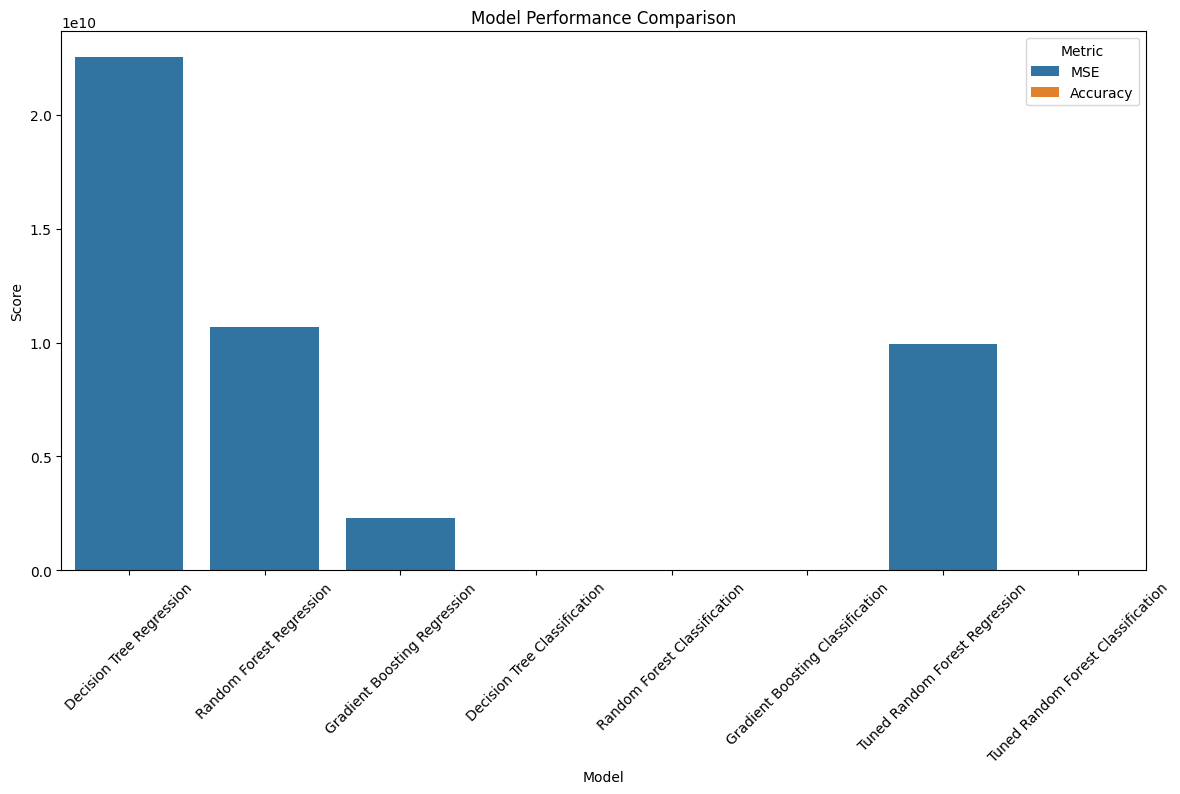
\includegraphics[width=0.7\textwidth]{assets/images/regression_performance.png}
    \caption{Model Performance Comparison for Regression}
    \label{fig:regression_performance}
\end{figure}

The Gradient Boosting Regression model outperformed the Decision Tree and Random Forest models, achieving the lowest MSE. The figure in \ref{fig:regression_performance} above shows the comparison of MSE across the models.


\begin{figure}[H]
    \centering
    \begin{subfigure}[H]{0.45\textwidth}
        \centering
        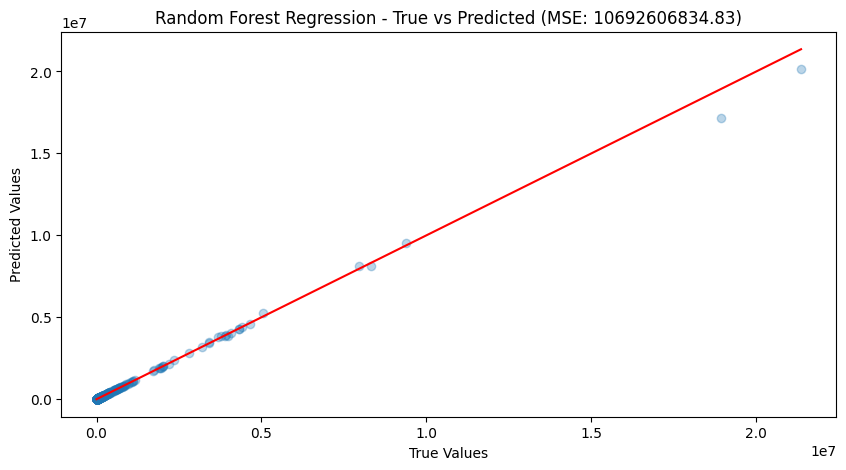
\includegraphics[width=\textwidth]{assets/images/random_forest_regression.png}
        \caption{Random Forest Regression - True vs Predicted Values}
        \label{fig:random_forest_regression}
    \end{subfigure}
    \hfill
    \begin{subfigure}[H]{0.45\textwidth}
        \centering
        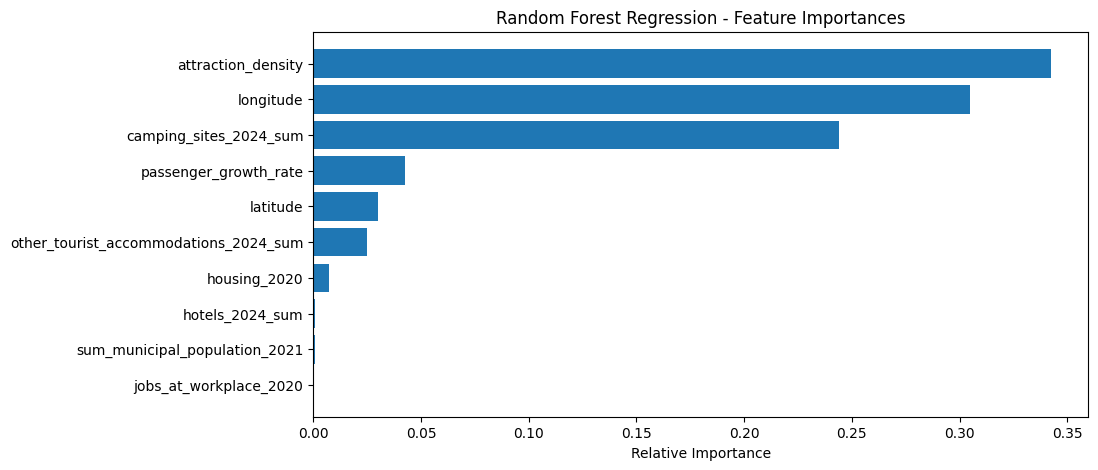
\includegraphics[width=\textwidth]{assets/images/feature_importance_random_forest.png}
        \caption{Feature Importance in Random Forest Regression}
        \label{fig:random_forest_feature_importance}
    \end{subfigure}
    \caption{Comparison of Random Forest Regression Results}
    \label{fig:random_forest_regression_comparison}
\end{figure}

Figure \ref{fig:random_forest_regression} shows the true vs predicted values for the Random Forest Regression model, indicating good alignment along the diagonal line. Figure \ref{fig:random_forest_feature_importance} highlights the most important features in the Random Forest Regression model, with \textit{attraction\_density} being the most significant.

\subsubsection{Classification}
The Random Forest Classification model was trained to predict whether a train station provides wifi service. We evaluated the model using the accuracy score metric.


\begin{figure}[H]
    \centering
    \begin{subfigure}[b]{0.3\textwidth}
        \centering
        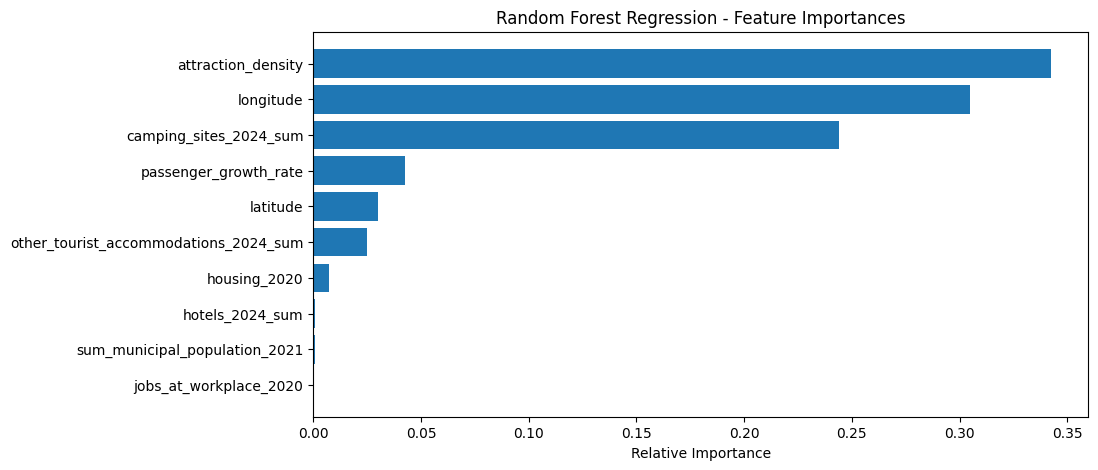
\includegraphics[width=\textwidth]{assets/images/random_forest_classification_feature_importance.png}
        \caption{Feature Importance for Random Forest Classification}
        \label{fig:random_forest_classification_feature_importance}
    \end{subfigure}
    \hfill
    \begin{subfigure}[b]{0.3\textwidth}
        \centering
        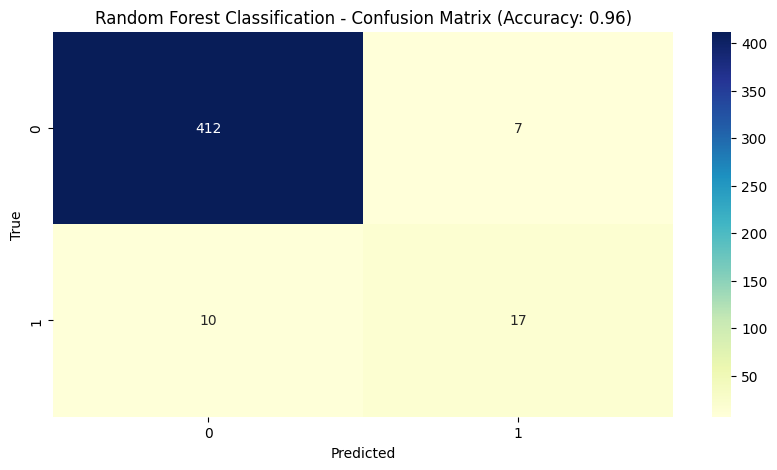
\includegraphics[width=\textwidth]{assets/images/random_forest_confusion_matrix.png}
        \caption{Confusion Matrix for Random Forest Classification}
        \label{fig:random_forest_classification_confusion}
    \end{subfigure}
    \hfill
    \begin{subfigure}[b]{0.3\textwidth}
        \centering
        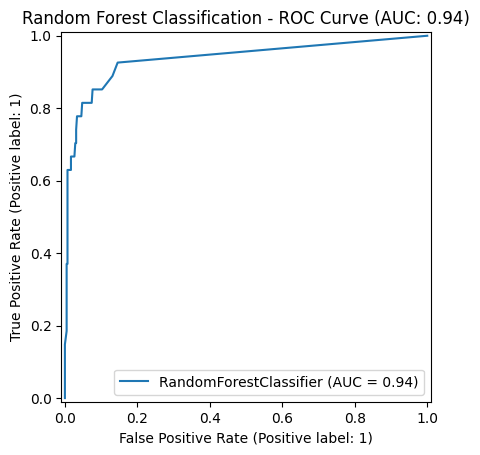
\includegraphics[width=0.75\textwidth]{assets/images/random_forest_ROC.png}
        \caption{ROC Curve for Random Forest Classification}
        \label{fig:random_forest_classification_ROC}
    \end{subfigure}
    \caption{Feature Importance, Confusion Matrix, and ROC for Random Forest Classification}
    \label{fig:classification_performance_and_confusion}
\end{figure}

The Random Forest Classification model achieved the highest accuracy compared to the Decision Tree and Gradient Boosting models. Figure \ref{fig:random_forest_classification_feature_importance} highlights the most important features used by the Random Forest Classification model. Figure \ref{fig:random_forest_classification_confusion} shows the confusion matrix for the Random Forest Classification model, indicating high accuracy. Figure \ref{fig:random_forest_classification_ROC} shows the ROC curve for the Random Forest Classification model, providing insights into the model's performance across different threshold settings. In the classification task, we faced class imbalance as the majority of the train stations do not provide wifi service. This was addressed using oversampling techniques to balance the classes and ensure that the model does not become biased towards the majority class.

\subsection{Hyperparameter Tuning}
To optimize the Random Forest models, we performed hyperparameter tuning using GridSearchCV. The best parameters for both regression and classification tasks were identified.

\subsection{Interpretation of Results}
The Gradient Boosting model showed the greatest performance in the regression task, while the Random Forest models demonstrated better performance in the classification task. Hyperparameter tuning further improved the performance of the Random Forest models, making them highly effective for both regression and classification.




